%------------------------------------------------------------------------------
\ifpdf
\graphicspath{{bild/}}
%{80_Bilder/PDF/}
%{80_Bilder/}}
\else
\graphicspath{%{80_Bilder/EPS/}
	%{80_Bilder/}
	{bild/}}
\fi
%%%%%%%%%%%%%%%%%%%%%%%%%%%%%%%%%%%%%%%%%%%%%%%%%%%%%%%%%%%%%%%%%%%%%%
%%%%%%%%%%%%%%%%%%%%%%%%%%%%%%%%%%%%%%%%%%%%%%%%%%%%%%%%%%%%%%%%%%%%%%


\chapter{Trajektorieplanung durch Lösung einer Randwertaufgabe}
\label{ch:Trajektorieplanung_durch_Lösung_einer_Randwertaufgabe}

Dieses Kapitel befasst sich mit der Trajektorieplanung von dem nichtlinearen System mittels des Python-Pakets \emph{PyTrajectory}. Im ersten Abschnitt geht es um die Vorstellung der allgemeinen Idee und den Algorithmen für die Trajektorieplanung mit dem Paket. In Abschnitt \ref{Erweiterung_der_Funktion_von_PyTrajectory} werden einige Probleme mit den Lösungen aus den Algorithmen diskutiert. Die simulierten Ergebnisse verschiedener Systeme werden auch in diesem Abschnitt vorgestellt.


\section{Grundlage zum Entwurf der Trajektorieplanung}
\label{Grundlage_zum_Entwurf_der_Trajektorieplanung}
\emph{PyTrajectory} ist ein Python Paket zum Trajektorien-Entwurf mit gegebenen Randwertbedingungen (Anfangs- und Endwerte der Systemzuständen sowie Eingängen) für nichtlineare Systeme. Hier wird die Grundlage über Trajektorienplanung grundsätzlich vorgestellt. Für weitere Informationen steht die Dokumentation der Software \cite{PyTra} zur Verfügung.
%%%%%%%%%%%%%%%%%%%%%%%%%%%%%%%%%%%%
\subsection{Kollokationsverfahren}
\label{Kollokationsverfahren}
Gesucht ist die Lösung $t\mapsto\vect{u}(t)$ des Randwertproblems:
\begin{eqnarray}
\vect{f}(\vect{x}(t), \vect{u}(t)) - \dot{\vect{x}} &=& \vect{0}, ~~t\in [0,T]
\label{eq:Kollocationverfahren}
\end{eqnarray}
mit dem Anfangswert $\vect{x}_{0} = \vect{X}_{a}$, Endwert $\vect{x}_{T} = \vect{X}_{b}$ an. $\dot{\vect{x}}$ ist die Ableitung nach der Zeit $t$, $\vect{X}_{a}\in \Reals^{n}, \vect{X}_{b}\in \Reals^{n}$ sind gegeben und $\vect{u}: \Reals\mapsto \Reals^{m}$ bezeichnet das gesuchte Eingangssignal. 

Das Zeitintervall $I = [0,T] $ kann wie Abb. \ref{fig:Collocation} unterteilt werden:
\begin{figure}
	\centering
	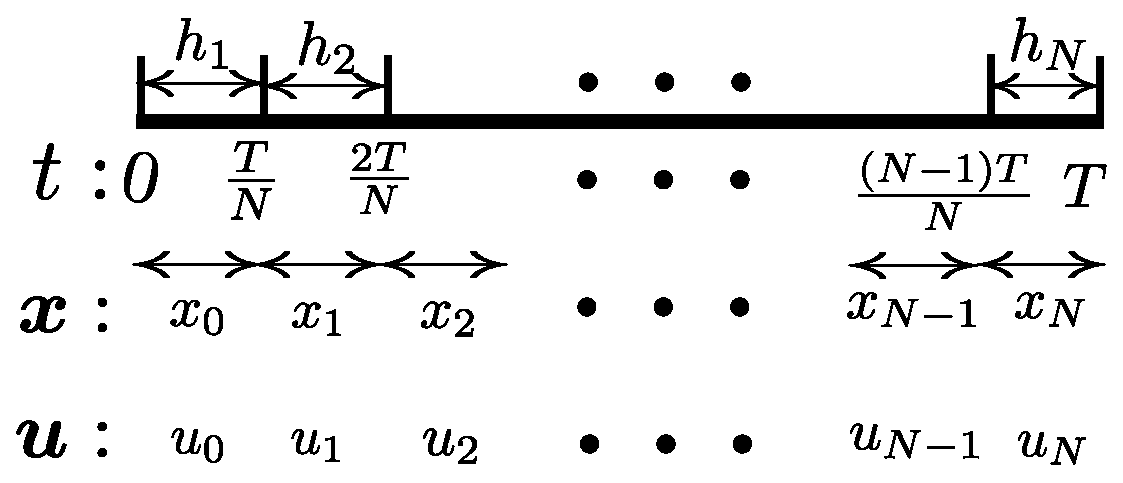
\includegraphics[width=7cm]{bild/modul/Collocation.eps}
	\caption[Kollokationsabschnitte $h_{i}$ und Kollokationspunkte $\vect{x}_{i}$, $\vect{u}_{i}$.]{Kollokationsabschnitte $h_{i}$ und Kollokationspunkte $\vect{x}_{i}$, $\vect{u}_{i}$: für jeden Abschnitt ist die Darstellung von $\vect{x}$ und $\vect{u}$ jeweils ein Polynom über $t$. Die Anzahlen der Splineabschnitte von $\vect{x}$ und $\vect{u}$ brauchen nicht äquivalent zu sein. (In dieser Abbildung sind sie als spezieller Fall gleich.)}
	\label{fig:Collocation}
\end{figure} 
 
Das Intervall $[0,T]$ wird in $N$ Teile mit gleichen Abstand eingeteilt ($h_{1} = h_{2} = \cdots = h_{N} = \frac{T}{N}$). Für jeden Abschnitt nimmt man eine Polynomfunktion dritten Grades jeweils für $\vect{x}$ und $\vect{u}$ an:
\begin{eqnarray}
\vect{S}_{x,i}(\vect{c},t) = \vect{x}_{i} &=& c_{xji0}+c_{xji1}\cdot (t-\frac{iT}{N_{x}}) + c_{xji2}\cdot (t-\frac{iT}{N_{x}})^{2} \notag\\&+& c_{xji3}\cdot (t-\frac{iT}{N_{x}})^{3}, ~~\scriptstyle{t\in [\frac{iT}{N_{x}}, \frac{(i+1)T}{N_{x}}),~~i= 0\cdots N_{x}-1, ~~j = 1\cdots n}\notag\\ 
\vect{S}_{u,i}(\vect{c},t) = \vect{u}_{i} &=& c_{uji0}+c_{uji1}\cdot (t-\frac{iT}{N_{u}}) + c_{uji2}\cdot (t-\frac{iT}{N_{u}})^{2} \notag\\&+& c_{uji3}\cdot (t-\frac{iT}{N_{u}})^{3}, ~~\scriptstyle{t\in [\frac{iT}{N_{u}}, \frac{(i+1)T}{N_{u}} ),~~i= 0\cdots N_{u}-1, ~~j = 1\cdots m}
\label{eq:form_von_Polynom_u_und_x}
\end{eqnarray}
Der Index $i$ und $j$ steht jeweils für den $i$-ten Abschnitt in Abb. \ref{fig:Collocation} und die $(j+1)$-te Komponente von $x$ bzw. $u$ (Da $\vect{x}/\vect{u}$ Vektor ist). $\vect{c}$ bedeutet Koeffizient der Polynomen. Es gibt insgesamt $4\cdot (N_{x}\cdot n + N_{u}\cdot m)$ Koeffizienten von $\vect{x}$ und $\vect{u}$ in $(N_{x}\cdot n + N_{u}\cdot m)$ kubischen Polynomfunktionen. 
 
Jetzt berücksichtigt man die Stetigkeit von $\vect{S}$. Die Polynomfunktionen sollen an der Abschnittsgrenzen zweimal stetig differenzierbar sein. Mit anderen Worten erfüllen sie in jeder Übergangsstelle folgende Formel:
\begin{eqnarray}
\vect{S}_{x/u,i}\left(\vect{c},t = \frac{iT}{N_{x}/N_{u}}\right ) &=& \vect{S}_{x/u,i+1}\left((\vect{c},t = \frac{iT}{N_{x}/N_{u}}\right )~~~~~~\text{(0.~Ableitung~stetig)}\notag\\
\dot{\vect{S}}_{x/u,i}\left(\vect{c},t = \frac{iT}{N_{x}/N_{u}}\right ) &=& \dot{\vect{S}}_{x/u,i+1}\left((\vect{c},t = \frac{iT}{N_{x}/N_{u}}\right )~~~~~~\text{(1.~Ableitung~stetig)}\notag\\
\ddot{\vect{S}}_{x/u,i}\left((\vect{c},t = \frac{iT}{N_{x}/N_{u}}\right ) &=& \ddot{\vect{S}}_{x/u,i+1}\left((\vect{c},t = \frac{iT}{N_{x}/N_{u}}\right )~~~~~~\text{(2.~Ableitung~stetig)}.\notag\\
\end{eqnarray}
Deswegen gibt es insgesamt $3((N_{x}-1)\cdot n + (N_{u}-1)\cdot m)$ Funktionen mit $(N-1)$ der Anzahl der Übergangsstellen. Mit dem Anfangs- und Endwert von $\vect{x}$ und $\vect{u}$ (insgesamt $2\cdot (n+m)$) werden $N_{cf} = (n\cdot (N_{x}+1) + m \cdot (N_{u}+1))$ freie Parameter $\vect{c}_{f}$ für Koeffizienten sichergestellt. Die anderen $N_{ca} = (n\cdot (3N_{x}-1) + m\cdot (3N_{u}-1))$ Parameter von Polynomen $\vect{c}_{a}$ hängen durch die obengenannten Funktionen von $\vect{c}_{f}$ ab.

Der freie Parametervektor $\vect{c}_{f}$ kann durch \eqref{eq:Kollocationverfahren} bestimmt werden. Dazu setzt man die Polynomform von $\vect{x}$ und $\vect{u}$ in Gl. \eqref{eq:Kollocationverfahren} ein und wählt man $(N_{t}+1)$ beliebigen Zeitpunkten\footnote{In \emph{PyTrajectory} wählt man Zeitpunkte mit festen Abstand: $t_{k} = \frac{kT}{N_{t}}, k = 0 \cdots N_{t}$.}:
\begin{eqnarray}
\vect{F\left (  \vect{c}_{f} \right )}&=&\begin{pmatrix}
\vect{f}\left ( \vect{S}_{x}\left ( \vect{c}_{f},t_{0} \right ), \vect{S}_{u}\left ( \vect{c}_{f},t_{0} \right ) \right )-\dot{\vect{S}}_{x}\left ( \vect{c}_f,t_{0} \right ) = \vect{0}\\
\vect{f}\left ( \vect{S}_{x}\left ( \vect{c}_{f},t_{1} \right ), \vect{S}_{u}\left ( \vect{c}_{f},t_{1} \right ) \right )-\dot{\vect{S}}_{x}\left ( \vect{c}_f,t_{1} \right ) = \vect{0}\\
\cdots  
\\
\vect{f}\left ( \vect{S}_{x}\left ( \vect{c}_{f},t_{N_{t}} \right ), \vect{S}_{u}\left ( \vect{c}_{f},t_{N_{t}} \right ) \right )-\dot{\vect{S}}_{x}\left ( \vect{c}_f,t_{N_{t}} \right ) = \vect{0}
\end{pmatrix}=\vect{0}\\ ~\text{mit}~~\vect{f}&:& \Reals^{N_{cf}}\mapsto \Reals^{n}\notag.
\label{eq:Gesamte_Funktion_von_KollocationVerfahren}
\end{eqnarray}
Die Dimension der unabhängigen Variablen $\vect{c}_{f}$ ist $N_{cf}$ und die Dimension von $\vect{F\left (  \vect{c}_{f} \right )}$ ist $n\cdot(N_{t}+1)$. Wenn die Anzahl der Variablen gleich oder größer als der Funktionen ist, wird mindestens eine exakte Lösung ausgerechnet. Das sichert die Funktionswerte zu den $(N_{t}+1)$ Zeitpunkten. Aber die Werte zu anderen Zeitpunkten können nicht garantiert werden.  Wie Abb. \ref{fig:Collocation_overdetermined} zeigt, liegt die Kurve $1$ zu den $(N_{t}+1)$ Zeitpunkten gerade auf der Achse, aber zu anderen Punkten liegt sie sehr weit von der Achse. Dagegen erhält die Kurve $2$ zu jedem Zeitpunkt zwar keine exakte Lösung, aber die Norm ist sehr klein. Deswegen sollte man für das Kollocationsverfahren eine überbestimmte Funktion auswählen, nämlich $n\cdot(N_{t}+1)>(n\cdot (N_{x}+1) + m \cdot (N_{u}+1))$.
\begin{figure}
	\centering
	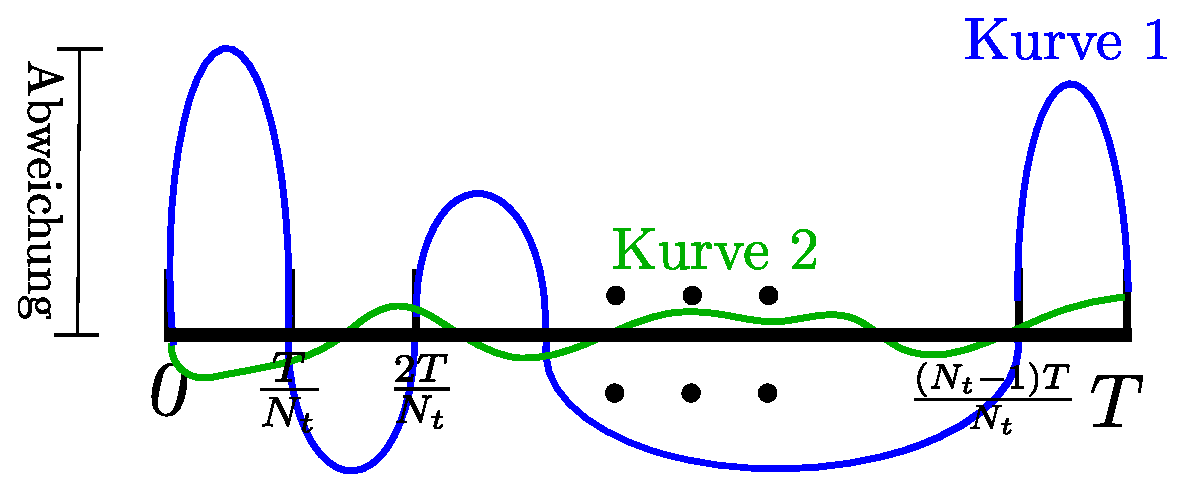
\includegraphics[width=8cm]{bild/modul/Collocation_overdetermined.eps}
	\caption[2 Trajektorienfälle von beispielsweise dem Systemzustand]{2 Trajektorienfälle von beispielsweise dem Systemzustand: aus Grund der Einfachheit ist $dim(\vect{x})=1$ gewählt. Die $y$-Achse ist die Abweichung zwischen der approximierten Lösung und dem idealen Fall. Zwar geht die Kurve $1$ zu den gewählten Zeitpunkten die $x$-Achse durch, aber sie hat eine viel größer Abweichung zu anderen Punkten als Kurve $2$.}
	\label{fig:Collocation_overdetermined}
\end{figure}  

Jetzt stellt sich die Frage: wie kann man eine optimale approximierte Lösung von der überdeterminierte Funktion (Gl. \eqref{eq:Gesamte_Funktion_von_KollocationVerfahren}) bestimmen? Das wird in nächsten Abschnitt beantwortet.
%%%%%%%%%%%%%%%%%%%%%%%%%%%%%%%%%%%%%%%%%%%%%%%%%%%%%%%%%
\subsection{Methode zur Lösung des Quadratmittelproblems}
\label{Methode_zur_Lösung_des_Quadratmittelproblems}
Das Quadratmittelproblem einer Funktionsvektor ist wie folgt definiert \cite{knorrenschild2017numerische}:
\begin{definition}[Quadratmittelproblem]
Gegeben ist ein Funktionsvektor\footnote{$n$ und $m$ hier sind anders wie die Dimensionen von $\vect{x}$ und $\vect{u}$ in letztem Abschnitt. $\vect{x}$ verweist nur die erforderlichen Parameter.}${\vect{F\left (\vect{x}\right )}}: \Reals^{n}\to \Reals^{m}$. Ein Vektor ${\vect{x}_{\ast}}$ ist zu finden, sodass die euklidische Norm des Funktionsvektors (oder: das ``zugehörige Fehlerfunktional'') minimiert wird:
\begin{eqnarray}
{\vect{x}_{\ast}} = \mathop {\argmin }\limits_{\vect{x}}\left | {\vect{F}}\left ( {\vect{x}} \right ) \right |_{2}^{2} = \mathop {\argmin }\limits_{\vect{x}}\left ( \sum_{i=1}^{m}\left ( f_{i}\left ( \vect{x} \right ) \right )^{2}\right )
\label{Def_LSP}\notag\\
\end{eqnarray}
mit $f_{i}: \Reals^{n}\to \Reals^{1}$. $\vect{x}_{\ast}$ hießt auch der stationäre Punkt.
\end{definition}
\subsubsection{Gauß-Newton-Verfahren}\label{Gauß-Newton-Verfahren}
%%%%%%%%%%%%%%%%%%%%%%%%%%%%%%%%%
Ein solches Quadratmittelproblem kann man mit verschieden Verfahren lösen. Eine typische Methode ist das Gauß-Newton-Verfahren (GN-Verfahren), das durch die lineare Approximation des nichtlinearen Problems löst. Mit der Ableitung erster Ordnung der Funktion $\vect{F(\vect{x})}$ konvergiert das Iterationsverfahren mit linearer Konvergenzordnung\footnote{Linear Konvergenzordnung bedeutet, dass $\norm{\vect{x}_{k+1} -\vect{x}_{\ast}} \leqslant \alpha \norm{\vect{x}_{k}-\vect{x}_{\ast}}$ mit $0 \leqslant \alpha \leqslant 1$.}. Im Folgenden geht die Methode mit der Taylorentwicklung von $\vect{F}$ und $f$ aus \cite{madsen2004methods}:
\begin{equation}
\begin{aligned}
f\left ( \vect{x}+\vect{h} \right ) &= f\left ( \vect{x} \right ) + f'\left ( \vect{x} \right )\cdot \vect{h} \overset{f' = \matr{J}}{=} f\left ( \vect{x} \right ) + \matr{J}\left ( \vect{x} \right )\cdot \vect{h} + o\left ( \vect{h}^{2} \right )\\
\vect{F}\left ( \vect{x}+\vect{h} \right ) &= f\left ( \vect{x}+\vect{h} \right )^ \mathrm{ T }\cdot f\left ( \vect{x}+\vect{h} \right )\approx \left ( f+\matr{J}\vect{h} \right )^ \mathrm{ T }\left ( f+\matr{J}\vect{h} \right )\\ &= f^ \mathrm{ T }f+2\vect{h}^ \mathrm{ T }\matr{J}^ \mathrm{ T }f + \vect{h}^ \mathrm{ T }\matr{J}^ \mathrm{ T }\matr{J}\vect{h} := \vect{G}\left ( \vect{h} \right ).\label{eq:Taylorentwicklung_von_GN_Verfahren}
\end{aligned}
\end{equation}
Das Symbol $\matr{J}$ steht für die Jacobi-Matrix. Nach der Ableitung des vorletzten Terms erhält man die 1. und 2. Ableitung von $\vect{G}$ bezüglich $\vect{h}$:
\begin{eqnarray}
\vect{G}'\left ( \vect{h} \right )  &=& 2\matr{J}^\mathrm{T}f + 2\matr{J}^\mathrm{T}\matr{J}\vect{h}\label{eq:G_1}\\
\vect{G}''\left ( \vect{h} \right ) &=& 2\matr{J}^\mathrm{T}\matr{J}.\label{eq:G_2}
\end{eqnarray}
Es wir angenommen, dass $\vect{G}''$ positiv definit ist\footnote{Das ist ein Nachteil von Gauß-Newton-Verfahren. Die Positivdefinitkeit kann nicht immer gesichert werden.}. Man definiert hier die Schrittweite $h=h_{\ast}$ als lokaler Minimum, wenn $\vect{G}'\left (\vect{h}_{\ast} \right ) = \vect{0}$ ist. Zur Berechnung von $\vect{h}_{\ast}$ wird Gl. \eqref{eq:G_1} gleich $0$ gesetzt:
\begin{equation}
\left ( \matr{J}^\mathrm{T} \matr{J} \right ) \cdot \vect{h}_{\ast}  = -\matr{J}^\mathrm{T}f.\label{eq:cal_NW_hs}
\end{equation}
Der stationäre Punkt $\vect{x}_{\ast}$ wird aus der vorherige Punkt $\vect{x_{\ast-1}}$ und $\vect{h}_{\ast}$ berechnet:
\begin{equation}
\vect{x}_{\ast} = \vect{x_{\ast-1}} + \vect{h}_{\ast} = \vect{x_{\ast-1}} - \left ( \matr{J}^\mathrm{T} \matr{J} \right )^\mathrm{-1} \cdot \matr{J}^\mathrm{T}f.\label{eq:newton-xs}
\end{equation} 
Neben der möglichen Nichtexistenz der inversen Matrix gibt es auch eine Beschränkung: mit der $\vect{x}_{\ast}$ durch das GN-Verfahren nicht gefunden kann, wenn der Anfangsschätzwert $\vect{x}_{0}$ nicht in der Näher von $\vect{x}_{\ast}$ liegt. Daher wird in nächsten Abschnitt eine andere Methode vorgestellt, damit man die obige Probleme vermeiden kann. 
\subsubsection{Levenberg-Marquardt-Algorithmus}
\label{Levenberg-Marquadt-Algorithmus}
%%%%%%%%%%%%%%%%%%%%%%%%%%%%%%%%%%%%%%%
Der nach Kenneth Levenberg und Donald Marquardt benannte Algorithmus ist tatsächlich eine Kombination von Methode des steilsten Abstiegs und Gauß-Newton-Verfahrens. Gl. \eqref{eq:LM_cal_hs} zeigt die detaillierte Form von Schrittweite $\vect{h}$ in LM-Algorithmus \cite{von2015einfuhrung}\cite{madsen2004methods}:
\begin{equation}
\left ( \matr{J}^\mathrm{T} \matr{J} + \mu\matr{I}\right ) \cdot \vect{h}  = -\matr{J}^\mathrm{T}f.
\label{eq:LM_cal_hs}
\end{equation}
$\matr{I}$ ist die Einheitsmatrix, $\mu$ ist ein ``Dämpfungsparameter''. Aufgrund der Existenz des Dämpfungparameters ist die Positivdefinitheit der Matrix $\matr{J}^\mathrm{T} \matr{J} + \mu\matr{I}$ gesichert. Falls $\mu$ groß ist (das passiert am Anfang der Iteration), ist die Funktion von der Schrittweite ähnlich wie Methode des steilsten Abstiegs, damit die Funktion bei $\vect{x}$ weit von Zielpunkt schnell konvergiert. Andernfalls verhält sich der LM-Algorithmus bei kleinem $\mu$ oder in der Umgebung von $\vect{x}_{\ast}$ wie NM-Verfahren aus. Das heißt, in den letzten Schritten konvergiert die Funktion auch schnell.

Ein wichtiger Teil für LM-Algorithmus ist die Bestimmung von Dämpfungsparameter $\mu$. Der Ausgangspunkt davon ist die Größe der Variable \emph{Verstärkungsverhältnis $\rho$}, die durch die Relation von der aktuellen Abnehme des nichtlinearen Systems in einem Schritt und der vorhergesagten Abnehme des linearisierten Systems definiert wird:  
\begin{eqnarray}
	\rho  = \frac{\left \|\vect{F}\left ( \vect{x} \right )\right \|^{2}-\left \| \vect{F}\left ( \vect{x}+\vect{h} \right )\right \|^{2}}{\left \| \vect{G}\left ( \vect{0} \right )\right \|^{2}-\left \| \vect{G}\left ( \vect{h} \right )\right \|^{2}} = \frac{\Delta F}{\Delta G}.
\label{eq:LM-Methode-rho}
\end{eqnarray}
Da $\vect{h}$ in die Richtung mit einer sinkenden Norm von $\vect{G}$ zeigt, soll der Wert von $\rho$ größer als $0$ sein. Wenn $\rho$ sehr klein oder $\Delta G$ viel größer als $\Delta F$ ist, ist der vorherige Schritt $\vect{h} = \min_{\vect{h}}{(\vect{G}(\vect{h}) + \frac{1}{2}\mu \vect{h}^{T}\cdot \vect{h})} $ zu groß und er muss im nächsten Schritt verkleinert werden. Das heißt, der Wert von $\mu$ muss vergrößert werden. Anderenfalls muss $\mu$ verkleinert werden, wenn der vorherige $\vect{h}$ zu klein (sonst kostet es mehrere Zeit, eine Lösung zu finden) ist. Ein typischer Entwurf von $\rho$ sieht wie folgendem Algorithmus:
\begin{algorithmic}
	%\centering
	\If {$\rho < 0.2$}
	\State $\mu_{new}: = \mu_{old} *2 $
	\ElsIf {$\rho > 0.8$}
	\State $\mu_{new}: = \mu_{old} / 2$
	\Else
	\State $\mu_{new} : = \mu_{old} $
	\EndIf
\label{Ag:dampfung_parameter}
\end{algorithmic}
                              
Setzt man Gl. \eqref{eq:Gesamte_Funktion_von_KollocationVerfahren} in Gl. \eqref{eq:LM_cal_hs} ein, ersetzt der Vektor $\vect{F(\vect{c}_{f})}$ hier $f$ und die freien Parameter $\vect{c}_{f}$ hier $\vect{x}$. Die Jacobi-Matrix $\vect{J}$ ist die Ableitungsmatrix von $\vect{F(\vect{c}_{f})}$ nach $\vect{c}_{f}$. Mit dem LM-Algorithmus wird eine optimale approximierte Lösung von $\vect{c}_{f}$ ausgerechnet. 

Nach der Iteration erhält man die optimalen freien Parameter, damit werden die Trajektorie von $\vect{u}(t)$ und $\vect{x}_{sp}(t)$ als Form der kubischen Polynom dargestellt wie Gl. \eqref{eq:form_von_Polynom_u_und_x}. Setzt man $\vect{u}(t)$ in den Zustandsgleichungen ein, wird auch ein $\vect{x}_{sim}(t)$ durch die Integration erstellt. Wenn die Abweichungen $1.)$ zwischen $\vect{x}_{sp}(t)$ und $\vect{x}_{sim}(t)$ und $2.)$ zwischen gegebenen Randwerte von $\vect{x}$ und $\vect{x}_{0}$, $\vect{x}_{T}$ unter den voraus gelieferten Beschränkungen nicht erfüllt werden, wird das System nochmal mit einer höheren Anzahl an Splineabschnitten gerechnet. Dieser Vorgang wird solange wiederholt, bis eine approximierte Lösung gefunden werden kann\footnote{Dieser Iterationsvorgang wird unter ``Hauptiteration'' genannt. Anders als die Iteration innerhalb des LM-Verfahrens (als Nebeniteration genannt)\label{Nebeniteraion} ist der Parameterwert nach einer Hauptiteration schon die optimale Lösung von LM-Verfahren, der aber die erforderte minimale Abweichung zwischen dem Soll- und Istendwert des Zustände überschreitet. Ein erneuter Iteraionsvorgang mit vergrößerten Anzahl der Splineabschnitte ist deswegen nötig.}.

Als Schluss dieses Abschnitts wird ein Beispiel mit \emph{PyTrajectory} gerechnet.

\begin{beispiel}[Einfacher Doppelintegrator mit \emph{PyTrajectory}]\label{bp:Dooelintegrator_ori}
 	Betracht man einen auf der X-Achse laufenden Wagen mit zwei Zustandskomponenten: die Verschiebung $x_{1}$ und die Geschwindigkeit $x_{2}$. Eine aufgeprägte Kraft wirkt auf den Wagen ein. Die Beschleunigung gilt als Systemeingang $u$. Die Systemgleichung lautet:
 	\begin{eqnarray}
 	\dot{x}_{1} &=& x_{2}\notag\\
 	\dot{x}_{2} &=& u.
 	\label{eq:Doppelintegrator}
 	\end{eqnarray}
 	
	Es sei gefordert, dass der Wagen sich von $0$ bis zu $1m$ bewegt und am Anfang und Ende in Ruhe ist. Mit anderen Worten ist der Anfangs- und Endwert von $x_{1}$ und $x_{2}$ jeweils ($0$,$1$) sowie ($0$,$0$). Die feste Überführungszeit ist $1$ Sekunde. 
	
	Die Anfangswerte der Parameter von dem \emph{PyTrajectory} ist wie folgt eingestellt: die Anfangsschätzwerte der freien Parameter für die Polynome $\vect{x}$ und $u$ als Form der Gl. \eqref{eq:form_von_Polynom_u_und_x} sind alle $0.1$, die Anfangszahl der Splineabschnitte für beide $\vect{x}$ und $u$ ist $2$. Falls nötig muss die Anzahl in dem nächsten Iteration verdoppeln.
	
	Abb. \ref{fig:Doppelintegrator_ohne_k_x} und Abb. \ref{fig:Doppelintegrator_ohne_k_u} zeigt die Simulationsergebnisse des Systems. Das System benötigt zwei Iterationen (nämlich endlich $4$ Spline-Abschnitte), um eine optimale Lösung von den freien Parameter $\vect{c}_{f}$ zu finden. Unter der Wirkung eines ungefähr sinusförmigen Eingangs mit maximal $6m/s^{2}$ läuft der Wagen entlang dem geplanten Weg. Das heißt, der Wagen beschleunigt sich in die ersten Halbzeit ($0.5s$), und nach der Erreichung der maximale Geschwindigkeit (circa $1.8m/s$) bremst er bis zum Stoppen.
	\begin{figure}[!h]
		\centering
		\includegraphics[width=0.7\linewidth]{bild/30_32/test0_ohne_k_ori_x.pdf} %13cm
		\caption[Trajektorie der Systemzustandskomponente $x_{1}$ und $x_{2}$ (Position und Geschwindigkeit).]{Trajektorie der Systemzustandskomponente $x_{1}$ und $x_{2}$ (Position und Geschwindigkeit). Die Überführungszeit ist fest: $1s$.}
		\label{fig:Doppelintegrator_ohne_k_x}
	\end{figure}
	
	
	
	\begin{figure}[!h]
		\centering
		\includegraphics[width=0.7\linewidth]{bild/30_32/test0_ohne_k_ori_u.pdf}%12cm
		\caption[Trajektorie des Systemeingangs $u_{1}$ (Wagenbeschleunigung).]{Trajektorie des Systemeingangs $u_{1}$ (Wagenbeschleunigung). Die Überführungszeit ist fest: $1s$.}
		\label{fig:Doppelintegrator_ohne_k_u}
	\end{figure}
\end{beispiel}

\section{Erweiterung der Funktion von PyTrajectory}
\label{Erweiterung_der_Funktion_von_PyTrajectory}
%%%%%%%%%%%%%%%%%%%%%%%%%%%%%%%%%%%%
Vor beginn der Arbeit war es möglich, eine Trajektorie von $\vect{u}$ und $\vect{x}$ eines Systems mithilfe des Pakets \emph{PyTrajectory} und der vom Nutzer voraus gelieferten Überführungszeit $T$ zu finden. Dabei könnten aber folgende Probleme auftreten: Einerseits wären die Systeme mit diesem $T$ nicht optimal (z.B. es bräuchte mehrmals Iterationen) , auf der anderen Seite kann bei manchen Systemen nur dann eine Trajektorie gefunden werden, wenn man zufällig die richtige Dauer gewählt hat. Deswegen liegt eine Aufgabe bei der Erweiterung der Funktion von PyTrajectory darin, eine geeignete Überführungszeit der Trajektorienplanung eines Systems ausrechnen zu lassen, anstatt sie vorgeben zu müssen.

\subsection{Optimale Überführungszeit}
\label{Optimale_Überführungszeit}
Es wird angestrebt, dass die Überführungszeit $T$ nicht vom Nutzer explizit vorgegeben wird, sondern anhand der Systemgleichungen mittels des Levenberg-Marquardt-Algorithmus automatisch ausgerechnet wird. Der Anfangspunkt ist die Ansetzung der Zeittransformation von $t = t$ zu $t = k\tau$, wobei $k$ ein zusätzlicher freier Parameter (ohne Einheit) ist. Dann folgt die Transformation:
\begin{eqnarray}
\dot{\vect{x}}_{\mathrm{ori}} &=& \frac{\mathrm{d} \vect{x}}{\mathrm{d} t} = \vect{f}\left ( \vect{x},t \right )\notag\\ %\label{eq:ori}\\
\dot{\vect{x}}_{\mathrm{new}} &=& \frac{\mathrm{d} \vect{x}}{\mathrm{d} \tau} = \frac{\mathrm{d} \vect{x}}{\mathrm{d} t}\cdot \frac{\mathrm{d} t}{\mathrm{d} \tau} = k\cdot \frac{\mathrm{d} \vect{x}}{\mathrm{d} t} = k\cdot \vect{f}(\vect{x},t) = \vect{f}_{\mathrm{new}}\left ( \vect{x},t,k \right ).\label{eq:mit_k}
\end{eqnarray}
Bei $k>1$ braucht das System mehr Zeit, um die Endposition zu erreichen und bei $k<1$ weniger. 

Nach der Implementierung in Python werden zwei Beispielsysteme damit getestet, um die Gültigkeit und Brauchbarkeit zu überprüfen. Für jedes Beispiel wird die unter der Berücksichtigung von Zeit entworfene Trajektorie (abgekürzt als ``Trajektorie mit k'') mit dem zum originalen System geeigneten Trajaktorie (Kurz als ``Trajektorie ohne k'') verglichen.
\begin{beispiel}[Doppelintegrator]\label{bp:Doppelintegrator_k}
	Die Ergebnisse für das System ``ohne k'' wurde schon im letzten Abschnitt vorgestellt. Die erweiterte Systemgleichung von dem System ``mit k'' sind:
	\begin{eqnarray}
	\dot{x}_{1} &=& k \cdot x_{2}\notag\\
	\dot{x}_{2} &=& k \cdot u.
	\label{eq:Doppelintegrator_mit_k}
	\end{eqnarray}
	
	Als Anfangswerte bleiben alle Parameter außer der Überführungszeit $T$ wie Bsp. \ref{bp:Dooelintegrator_ori} unverändert. $T$ hängt von der freie Variable $k$ mit dem Anfangsschätzwert $k_{0}=1.23$ ab.
	
	\textbf{Einstellung von Anfangswerte der freien Parameter $\vect{c}_{f}$ als $\vect{0.1}$:}~~Der Wagen bewegt noch von $0$ bis zu $1m$ und am Anfang und Ende bleibt er in Ruhe. Die Anfangsschätzwerte von $\vect{c}_{f}$ sind noch $0.1$, die Anzahl der Spline-Abschnitt am Beginn des Algorithmus und der entsprechende Multiplikator für die Iteration sind jeweils noch $2$. 
	
	Mehr als in der Randwertaufgabe-Lösung mit den originalen Systemgleichungen benötigt das erweitere System $4$ Hauptiterationen\footnote{Die Erklärung für Haupt- und Nebeniteration liest man \ref{Nebeniteraion}.} (also $16$ Spline-Abschnitte), um eine optimale Lösung von $\vect{c}_{f}$ zu finden.
	
	Aus Abb. \ref{fig:Doppelintegrator_mit_k_x} und Abb. \ref{fig:Doppelintegrator_mit_k_u} kann man erkennen, zwar die maximale Kraft und die Geschwindigkeit weit kleiner als die im originalen System sind, ist aber der Wert von $k$ ist hier ziemlich groß (ungefähr $1662,53$)! Der Wert von $k$ nimmt ab $1.23$ in jeden Iteration zu. Der Wagen in diesem Beispiel muss sich deshalb $1662s$ lang bewegen, bevor er in die Endposition ankommt. Das bedeutet, die Lösung von $k$ ist zwar \textbf{richtig} aber \textbf{nicht brauchbar}.
	\begin{figure}[!h]
		\centering
		\includegraphics[width=0.7\linewidth]{bild/30_32/test0_mit_k_ori_x.pdf}%13cm
		\caption[Verlauf der Systemzustände vom System \eqref{eq:Doppelintegrator_mit_k}.]{Verlauf der Systemzustände vom System\eqref{eq:Doppelintegrator_mit_k}. $x_{1}$ und $x_{2}$ stehen für Position und Geschwindigkeit. Anfangswerte der freien Spline-Parameter sind alle $0.1$. Die $x$-Achse steht nicht für die reale Überführungszeit, die tatsächlich $(1\cdot k)$ Sekunde dauert.}
		\label{fig:Doppelintegrator_mit_k_x}
	\end{figure}
	\begin{figure}[!h]
		\centering
		\includegraphics[width=0.7\linewidth]{bild/30_32/test0_mit_k_ori_u.pdf}%13cm
		\caption[Verlauf des Systemeingangs und die Veränderungskurve von $k$ vom System \eqref{eq:Doppelintegrator_mit_k}.]{Verlauf des Systemeingangs und die Veränderungskurve von $k$ vom System \eqref{eq:Doppelintegrator_mit_k}. $u_{1}$ stehen für Wagenbeschleunigung. Der Wert von $k$ steigt immer an. Anfangswerte der freien freien Parameter sind alle $0.1$. Es gibt insgesamt ungefähr $2000$ Nebeniterationen. Die ``Iteraion'' in der Abbildung von $k$ ist tatsächlich Nebeniteration (im Folgenden ebenso).}
		\label{fig:Doppelintegrator_mit_k_u}
	\end{figure}
	
	\textbf{Einstellung von Anfangswerte der freien Parameter $\vect{c}_{f}$ aus dem Simulationsergebnis der originalen Systemgleichungen:}~~Zur Verbesserung des Ergebnisses wird ein anderer Anfangswert für die Splineparameter gewählt. Statt aller Werte $0.1$ sind die freien Parameter jetzt gleich den Rechenergebnissen der Splineparameter nach der ersten Iteration in dem System ``ohne k''. Die Kurven in Abb. \ref{fig:Doppelintegrator_mit_k_x_aus} und \ref{fig:Doppelintegrator_mit_k_u_aus} sehen besser als in Abb. \ref{fig:Doppelintegrator_mit_k_x} und Abb. \ref{fig:Doppelintegrator_mit_k_u} aus. In dem ganzen Iterationsverlauf steigt der Wert von $k$ hauptsächlich mit $2$-mal Abstieg (bei der ersten und siebten Iteration). Im Vergleich zu dem Simulationsergebnis mit allen Anfangswerten $0.1$ braucht diese nur zwölf Nebeniterationen. Der Wagen stoppt zum Zeitpunkt $1.67$s. 
	
	\begin{figure}[!h]
		\centering
		\includegraphics[width=0.7\linewidth]{bild/30_32/test0_mit_k_Ite1_x.pdf}%13cm
		\caption[Trajektorie der Systemzustandskomponente vom System \eqref{eq:Doppelintegrator_mit_k}.]{Trajektorie der Systemzustandskomponente vom System \eqref{eq:Doppelintegrator_mit_k}. Anfangswerte von $\vect{c}_{f}$ sind aus den Ergebnissen von originalen Systemgleichungen (ohne k) gegeben.}
		\label{fig:Doppelintegrator_mit_k_x_aus}
	\end{figure}

	\begin{figure}[!h]
		\centering
		\includegraphics[width=0.7\linewidth]{bild/30_32/test0_mit_k_Ite1_u.pdf}%13cm
		\caption[Trajektorie des Systemeingangs vom System \eqref{eq:Doppelintegrator_mit_k}.]{Trajektorie des Systemeingangs vom System \eqref{eq:Doppelintegrator_mit_k}. Anfangswerte von $\vect{c}_{f}$ sind aus den Ergebnissen von originalen Systemgleichungen gegeben.}
		\label{fig:Doppelintegrator_mit_k_u_aus}
	\end{figure}
	
\end{beispiel}

Dieses Beispiel zeigt eine starke Abhängigkeit der Konvergenz des Levenberg-Marquardt-Algorithmus von den Anfangsschätzwerten. Wenn die Anfangsschätzwerte der Parameter zu weit von der unbekannten Minimalstelle vorgegeben werden, kann die Lösung des Quadratmittelproblems eines Regelsystems mittels LM-Algorithmus nicht konvergieren oder erreicht nur einen lokalen, nicht global optimierten Punkt.

Das folgende Beispiel stellt die Anwendung der LM-Methode in einem verbreiterten nichtlinearen System vor.

\begin{beispiel}[Inverses-Pendel-System]\label{bp:Inverses_Pendel_System}
	Abb. \ref{fig:Inverses-Pendel} zeigt das Schema des inversen Pendels. Der Pendelarm ist auf einem horizontal bewegten Wagen montiert. Der Wagen bringt daher eine horizontale Kraft auf das Pendel auf. Beim Aufprägen der Kraft ${F}$ auf den Wagen bewegt sich das Pendel von unten nach oben. Die instabile Ruhelage ist der Punkt, in dem das Pendel genau senkrecht zum Wagen steht und der Drehwinkel $180^{\circ}$ beträgt. Systemvariable in diesem Modell sind die Wagenposition ${x}_{1}$, dessen Geschwindigkeit ${x}_{2}$, der Pendeldrehwinkel ${x}_{3}$, die Drehgeschwindigkeit davon ${x}_{4}$. Der einzige Systemeingang ist die auf den Wagen aufgeprägte Kraft $u=f_{w}$.
	\begin{figure}
		\centering
		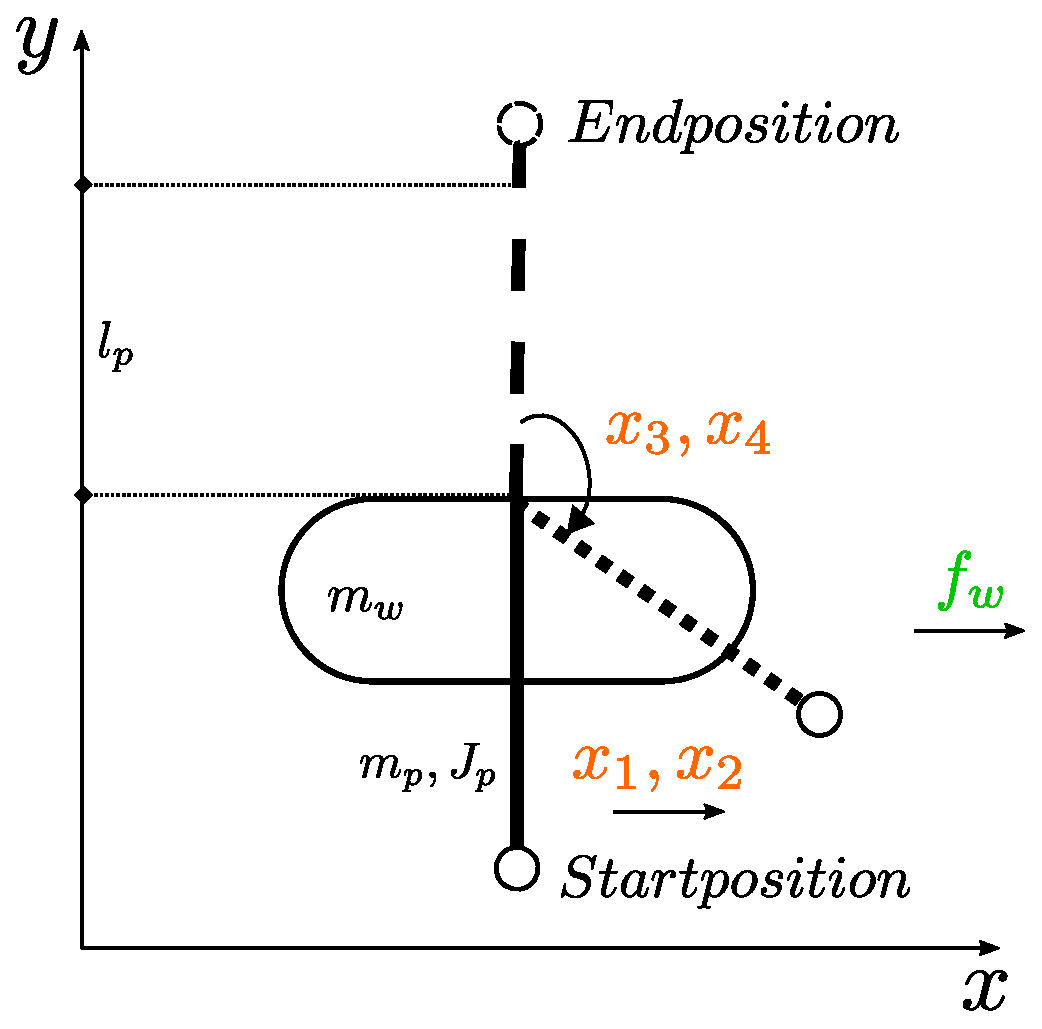
\includegraphics[width=6cm]{bild/modul/Inverses-Pendel.eps}
		\caption[Struktur des inversen Pendels.] {Struktur des inversen Pendels: in dem System gibt es vier Zustände ${x}_{1}$ bis ${x}_{4}$. Das Pendel bewegt sich von $180^{\circ}$ bis zur instabilen Ruhelage (nämlich vom ganz unten zu ganz oben). $m_{w}$ und $m_{p}$ sind jeweils die Masse des Wagens und des Pendels, $J_{p}$ ist das Trägheitsmoment und $l_{p}$ ist der Abstand zwischen dem Stützpunkt und dem Pendelschwerpunkt. Die Pfeile neben Zuständen geben die Vektorrichtung an. $x$ und $y$ sind Koordinatenachsen.}
		\label{fig:Inverses-Pendel}
	\end{figure}  

	Die dazugehörenden Differentialgleichungen des Modells sind wie folgt beschrieben \cite{kunze2016pytrajectory}:
	\begin{eqnarray}
	\dot{x}_{1}&=&x_{2}\notag\\
	\dot{x}_{2}&=&\frac{m_{p}\sin(x_{3})(-l_{p}x_{4}^{2}+g\cos(x_{3}))}{m_{w}l_{p}+m_{p}\sin^{2}(x_{3})}+\frac{\cos(x_{3})}{m_{w}l_{p}+m_{p}l_{p}\sin^{2}(x_{3})}u\notag\\
	\dot{x}_{3}&=&x_{4}\notag\\
	\dot{x}_{4}&=&\frac{\sin(x_{3})(-m_{p}l_{p}x_{4}^{2}\cos(x_{3})+g(m_{w}+m_{p}))}{m_{w}l_{p}+m_{p}\sin^{2}(x_{3})}+\frac{\cos(x_{3})}{m_{w}l_{p}+m_{p}\sin^{2}(x_{3})}u.\label{eq:DLG_Inverses_Pendel_compact}   
	\end{eqnarray}
	
	Wenn die Wagenverschiebung $x_{1}$ als der Systemausgang gewählt wird, lässt sich die Systemzustandsdarstellung mit der Ein-Ausgang-Linearisierung einfacher beschreiben. Da der Systemausgang $y = x_{1}$ und $\dot{y} = \dot{x}_{1} = x_{2}$ sowie $\ddot{y} = \dot{x}_{2} = M_{1}(\vect{x})+ M_{2}(\vect{x})\cdot u$ ist, ersetzt ein virtueller Eingang $v$ mit $\dot{x}_{2} = v$ den originale Systemeingang $u$ in den Systemgleichungen und erhält man:  
	\begin{eqnarray}
	\dot{x}_{1}&=&x_{2}\notag\\
	\dot{x}_{2}&=&u\notag\\
	\dot{x}_{3}&=&x_{4}\notag\\
	\dot{x}_{4}&=&\frac{g}{l_{p}}\sin(x_{3})+\frac{1}{l_{p}}\cos(x_{3})u.\label{eq:DLG_Inverses_Pendel_partiell_lin}   
	\end{eqnarray}
	
	Die Verfahrensparameter sind wie folgt eingestellt: weil der Pendel sich von unten nach oben drehen und der Wagen endlich zum Startpunkt zurückgehen soll, sind die Randwerte von $\vect{x}$ wie $\left ( 0,0,\pi ,0 \right )\rightarrow \left ( 0,0,0,0 \right )$ erfordert. Die Anfangszahl der Spline-Abschnitte und das Iterationsvielfache sind jeweils $2$. Alle Anfangsschätzwerte der Polynomkoeffizienten sind $0.1$. Der Anfangswert von $k$ für das System mit der Wirkung von $k$ ist noch $1.23$. Die Ergebnisse sind in Abb. \ref{fig:Inverses_Pendel_ohne_k_x}, Abb. \ref{fig:Inverses_Pendel_ohne_k_u}, Abb. \ref{fig:Inverses_Pendel_mit_k_x_ori} und Abb. \ref{fig:Inverses_Pendel_mit_k_u_ori} dargestellt.
	
	\begin{figure}
		\centering
		\includegraphics[width=0.8\linewidth]{bild/30_32/example0_ohne_k_x.pdf}%13cm
		\caption{Verlauf der Zustandsparameter des inversen Pendel System (ohne $k$) mit dem virtuellen Eingang.}
		\label{fig:Inverses_Pendel_ohne_k_x}
	\end{figure}

	\begin{figure}[!h]
		\centering
		\includegraphics[width=0.7\linewidth]{bild/30_32/example0_ohne_k_u.pdf}%12cm
		\caption[Verlauf des virtuellen Eingangs des inversen Pendel System (ohne $k$).]{Verlauf des virtuellen Eingangs des inversen Pendel System (ohne $k$). Die maximale Geschwindigkeit von $u$ ist ungefähr $28m/s^{2}$.}
		\label{fig:Inverses_Pendel_ohne_k_u}
	\end{figure}

	\begin{figure}[!h]
		\centering
		\includegraphics[width=0.8\linewidth]{bild/30_32/example0_mit_k_x_ori.pdf}%13cm
		\caption{Systemzustandskurven des inversen Pendel System (mit $k$) mit dem virtuellen Eingang.}
		\label{fig:Inverses_Pendel_mit_k_x_ori}
	\end{figure}
	
	\begin{figure}[!h]
		\centering
		\includegraphics[width=0.7\linewidth]{bild/30_32/example0_mit_k_u_ori.pdf}%13cm
		\caption[Systemeingang des inversen-Pendels (mit k) mit dem virtuellen Eingang.]{Systemeingang des inversen-Pendels (mit k) mit dem virtuellen Eingang. Die maximale Beschleunigung trägt ca. $12m/s^{2}$ und nur Hälfte des Wertes in Abb. \ref{fig:Inverses_Pendel_ohne_k_u}.}
		\label{fig:Inverses_Pendel_mit_k_u_ori}
	\end{figure}
	
	Nach 5 Iterationen (also 32 Spline-Abschnitte) rechnen beide Systeme optimale Lösungen aus. Wie in Abb. \ref{fig:Inverses_Pendel_mit_k_x_con} schwingt der Wert von $k$ (nicht monotone Abbildung) und endet um $1.48$, was als plausibler Wert erscheint. Für das System ohne oder mit der Wirkung von $k$ sind die Kurvenformen von Zustandsvariablen und dem virtuellen Eingang fast identisch. Aber Offensichtlich liefert die Trajektorie für das System mit $k$ einen kleineren Bewegungsbereich für $\vect{x}$ und $u$ (z.B. $x_{2}$ läuft jeweils $(-2~\text{bis}~+4)m/s$ im System ohne Zeittransformation und $(-2~\text{bis}~+2.5)m/s$ mit den geänderten Koordinaten). Deswegen wird weniger Eingangsenergie im letzteren System benötigt. In Bezug auf den relativ kleinen Unterschied bei der Überführungszeit ($1$s und $1.48$s) ist die Trajektorieplanung für das System mit der Wirkung von $k$ besser.
	
	Jetzt wird ein anderer Vorteil von System mit k diskutiert. Wie würde sich die Trajektorieplanung verändern, wenn auf die Systemzustände eine Beschränkung ausgeübt würde? Als ein Testzustand wählt man hier die Wagenverschiebung $x_{1}$. Aus Abb. \ref{fig:Inverses_Pendel_ohne_k_x} und \ref{fig:Inverses_Pendel_mit_k_x_ori} ist der Bewegungsbereich von $x_{1}$ jeweils $(-0.42~\text{bis}~+0.5)m$ und $(-0.58~\text{bis}~+0.3)m$, deswegen kann man eine Beschränkung für $x_{1}$ als einen zusätzlichen Bedingung des Systems einstellen: der Wagen bewegt nur im Bereich von $(-0.2~\text{bis}~+0.4)$m. Nach acht Iterationen rechnet das System mit $k$ eine Lösung: $k=1.0535$ aus, dennoch kann das originale System bis zur achten Iteration kein Ergebnis erhalten.
	
	
	
	\begin{figure}[!h]
		\centering
		\includegraphics[width=0.8\linewidth]{bild/30_32/example0_mit_k_x_con.pdf}%13cm
		\caption[Zustandsvariablenkurven des inversen-Pendels (mit k) mit dem virtuellen Eingang.]{Zustandsvariablenkurven des inversen-Pendels (mit k) mit dem virtuellen Eingang. $x_{1}$ ist zwischen ($-0.2$, $0.4$) eingeschränkt.}
		\label{fig:Inverses_Pendel_mit_k_x_con}
	\end{figure}
	
	\begin{figure}[!h]
		\centering
		\includegraphics[width=0.7\linewidth]{bild/30_32/example0_mit_k_u_con_makersize=10.pdf}%13cm
		\caption[Systemeingangskurve des inversen-Pendels (mit k) mit dem virtuellen Eingang.]{Systemeingangskurve des inversen-Pendels (mit k) mit dem virtuellen Eingang. $x_{1}$ ist zwischen ($-0.2$, $0.4$) eingeschränkt.}
		\label{fig:Inverses_Pendel_mit_k_u_con}
	\end{figure}

\end{beispiel}

Zusammengefasst aus oberen Beispielen stellt man eine Hypothese auf: Die Trajektorie kann für breitere/strengere Situationen/Bedingungen unter Berücksichtigung der Ausrechnung von einer geeigneten Überführungszeit eingeplant werden, sofern gute Anfangswerte der freien Splineparameter $\vect{c}_{f}$ vorgegeben werden. Die Richtigkeit dieser Idee wird im nächsten Abschnitt diskutiert.

\subsection{Einfluss der Startschätzung von $\vect{c}_{f}$}
\label{Einfluss_der_Startschätzung_von_cf}
Wie in Abb. \ref{fig:SA} findet der Levenberg-Marquardt-Algorithmus zum Lösen des Quadratmittelproblems nur lokale Minimum auf. Mit verschiedenen Anfangsschätzwerten werden wahrscheinlich unterschiedlichen Ergebnisse von $\vect{c}_{f}$ ausgerechnet. Das Paket \emph{PyTrajectory} stellt eine Möglichkeit zur Verfügung, $\vect{c}_{f}$ gemäß der Vorgabe eines Saat-Wertes (engl. seed) mit pseudo-zufälligen Werten im halboffenen Intervall $[0.0, 1.0)$ festzulegen.

Zum Überprüfen der Hypothese wählt man den Saat-Wert von $0$ bis $99$ für den Doppelintegrator, das inversen Pendel und einen zwei-Gelenke-Manipulator System (siehe Anhang \ref{Ausgang_Zwei_Gelenke_Manipulator} für die Systemdarstellung). Hier berücksichtigt man außer der Situation in Beispiel \ref{bp:Inverses_Pendel_System} (Inverses-Pendel-System-A) noch eine Trajektorienplanung für das inversen-Pendel-System mit der Randwerte von $\vect{x}$: $\vect{x}_{0}=(0,0,0,0)$ und $\vect{x}_{0}=(0,0,\pi,0)$ (Inverses-Pendel-System-B)\footnote{Für dieses System kann kein geeignetes $k$ mit den Startschätzwerte $\textbf{0.1}$ ausgegeben werden.}. Aus den vorher gezeigten Ergebnissen ist schon bekannt, dass bei allen Startschätzwerten gleich $0.1$ gilt $k_{end}=1662$ bei dem Doppelintegrator System und $k_{end}=1.48$ bei dem inversen Pendel System, wenn sich das Pendel von unten nach oben dreht. Für beide Systeme ist die maximale Iterationsanzahl $6$ (oder $64$ Spline-Abschnitten.)

Abb. \ref{fig:SA} stellt die statistischen Daten mit $100$ Saat-Werten dar. Bei dem Doppelintegrator System ist es interessant, dass in $92\%$ Fällen eine Losung von $k$ ausgerechnet werden kann, die aber sehr ähnlich zueinander und zu den Ergebnissen bei $\vect{c}_{f}=\vect{0.1}$ ist $(1660)$. In den restlichen $8$ Fällen hat $k$ bis sechsten Iteration auch einen ähnlichen Wert $(-1660)$. Für das inverse-Pendel System mit dem von oben nach unten drehenden Pendel, egal welche Anfangswerte eingestellt werden, findet der Rechner keinen plausiblen Wert von $k_{end}$. Das ist gleich wie der Fall $\vect{c}_{f}=\textbf{0.1}$. Aber für das Beispiel \ref{bp:Inverses_Pendel_System} sind die Lösungen von $k$ mit allen Saat-Werten ungefähr identisch: $k \approx 0$. Da der Wert von $k$ immer so klein ist, ist es anzunehmen, mit mehreren Iterationen auch keine Lösung gefunden wird. Bei dem Zwei-Gelenke-Manipulator funktioniert die Idee aber sehr gut. Deutlich hängt der Erfolg des Algorithmus zum Ausfinden eines brauchbaren $k$ von der Anfangswerten ab.


\begin{figure}[!h]
	\centering
	\begin{subfigure}[t]{0.45\textwidth}%
		\centering
		\label{fig:SA_for_Doppelintegrator}
		\includegraphics[width=0.7\linewidth]{bild/30_32/Doppelintegrator.png}
		\subcaption{Die benötigten Spline-Abschnitten für den Doppelintegrator}	
	\end{subfigure}
	%\hfill
	\begin{subfigure}[t]{0.45\textwidth}%
		\centering
		\label{fig:SA_for_zwei_Gelenk_Manipulator}
		\includegraphics[width=0.7\linewidth]{bild/30_32/2_Gelenke_Manipulator.png}
		\subcaption{Die benötigten Spline-Abschnitten für den zwei-Gelenke-Manipulator}
	\end{subfigure}
	\bigskip 
	\begin{subfigure}[t]{0.45\textwidth}%
		\centering
		\label{fig:SA_for_inversen_Pendel_ori}
		\includegraphics[width=0.7\linewidth]{bild/30_32/Inverses-Pendel-A.png}
		\subcaption{Die benötigten Spline-Abschnitten für das Inverses-Pendel-System-A.}
	\end{subfigure}
	%\hfill
	\begin{subfigure}[t]{0.45\textwidth}%
		\centering
		\label{fig:SA_for_inversen_Pendel_inverse}
		\includegraphics[width=0.7\linewidth]{bild/30_32/Inverses-Pendel-B.png}
		\subcaption{Die benötigten Spline-Abschnitten für Inverses-Pendel-System-B.}
	\end{subfigure}
	\caption[Vergleich des Spline-Abschnittsanzahls mit unterschiedlichen Startschätzwerte von $\vect{c}_{f}$.]{Vergleich des Spline-Abschnittsanzahls mit unterschiedlichen Startschätzwerte von $\vect{c}_{f}$. {SA} ist die Abkürzung für Spline-Abschnittszahl. Das erste Element in der Klammer steht für die echte Rechenzeit des Rechners. Das zweite ist der Modalwert von $k_{end}$.}
	\label{fig:SA}
\end{figure}


Aus dem Beispiel ist die Einstellung der Anfangswerte von freien Parameter mittels des Saat-Wertes für einige Regelsysteme geeignet. Aus der Sicht der Autorin liegt der Grund vermutlich in den Startwerte, die beliebig ausgewählt werden und noch weit von ihren tatsächlichen optimalen Werte liegen.

Die Vorgabe guter Startwerte für $\vect{c}_{f}$ ist also nicht einfach, deswegen werden einige andere Methoden zur Verbesserung der Lösung von $k$ entworfen.
 
Zuerst versucht man den Wert von $k$, in einem gegebenen zu beschränken. % wird eine Straffunktion von k zur Verbesserung des Überführungszeitalgorithmus entworfen, 

\subsection{Beschränken des Wertbereichs von $k$}
\label{Beschränken_des_Wertbereichs_von_k}
Die prinzipielle Idee kommt aus der Beschränkung von Systemzustände, die in \emph{PyTrajectory} schon realisiert wird. Der Ausgangspunkt liegt in der Transformation der Darstellung von der freien Variable $k$ von der originalen Systemkoordinaten mittels einer monotonen steigenden Sättigungsfunktion $\psi$ in einen neuen Koordinaten, darin keine Begrenzung von dem neuen $k$ besitzt. $k$ in der neuen Koordinate wird wie ``$\kappa$'' genannt und wie folgt geschrieben:
\begin{eqnarray}
k^{-}\leq k = \psi (\kappa,k^{\pm}) = k^{+}- \frac{k^{+}-k^{-}}{1+e^{m\cdot \kappa}}\leq k^{+},~~m := \frac{4}{k^{+}-k^{-}}.
\label{eq:Saturation_function}
\end{eqnarray}
Gl. \eqref{eq:Saturation_function} bedeutet, dass $k$ in $k^{+}$ und $k^{-}$ beschränkt wird. Die Ableitung von $\psi$ nach $\kappa$:
\begin{eqnarray}
\frac{\mathrm{d} \psi}{\mathrm{d}\kappa} = \frac{m(k^{+}-k^{-})e^{m\cdot sk}}{(1+e^{m\cdot \kappa})^{2}} = \frac{4\cdot e^{m\cdot \kappa}}{(1+e^{m\cdot \kappa})^{2}}
\label{eq:Saturation_function_diff}
\end{eqnarray}
ist immer positiv. $k$ wird durch $\kappa$ in den Systemfunktionen ersetzt und der Wert von $\kappa$ wird mittels des Levenberg-Marquadt-Algorithmus ausgerechnet. Nach der Erhaltung von $\kappa$ weißt man dann die Größe von $k$. Die Kurve von $\psi$ ist wie Abb. \ref{fig:psi_plot} dargestellt. Siehe \cite{graichen2006inversionsbasierter} und \cite{kunze2016pytrajectory} für weitere Information.
\begin{figure}[!h]
	\centering
	\includegraphics[width=0.7\linewidth]{bild/30_32/psi.png}%13cm
	\caption{Die Kurve der Sättigungsfunktion $\psi$ mit $k^{+}=6.0$ und $k^{-}=-6.0$.}
	\label{fig:psi_plot}
\end{figure}
Zur Überprüfung dieser Idee stellt man zuerst $k^{+}=5$ und $k^{-}=0$ in dem Doppelintegrator System (Beispiel \ref{bp:Doppelintegrator_k}) ein. Der Anfangsschätzwert von $k$ ist noch $1.23$. Das damit berechnete Ergebnis wird in Abb. \ref{fig:Doppelintegrator_mit_k_constrain_sk_5} gezeigt.

\begin{figure}[!h]
	\centering
	\includegraphics[width=0.7\linewidth]{bild/30_32/test0_mit_k_con_sk_5.pdf}
	\caption[Die Entwicklung von $\kappa$ in der transformierten Koordinaten und von $k$ in der originalen Koordinaten für das Doppelintegrator System.]{Die Entwicklung von $\kappa$ in der transformierten Koordinaten und von $k$ in der originalen Koordinaten für das Doppelintegrator System. Der Wert von $\kappa$ ist nicht begrenzt während $k$ hier innerhalb von ($0-5$) bleiben muss.}
	\label{fig:Doppelintegrator_mit_k_constrain_sk_5}
\end{figure}
\begin{figure}[!h]
	\centering
	\includegraphics[width=0.7\linewidth]{bild/30_32/test0_mit_k_con_sk_30.pdf}%width=13cm
	\caption[Die Entwicklung von $\kappa$ und $k$ für Doppelintegrator System.]{Die Entwicklung von $\kappa$ und $k$ für Doppelintegrator System. $k$ muss jetzt innerhalb von ($0-30$) bleiben.}
	\label{fig:Doppelintegrator_mit_k_constrain_sk_30}
\end{figure}
Dieses System benötigt $2$ Iterationen, eine Lösung zu finden. Schließlich ist $k=4.999$ und nähert der Obergrenze. Bei der zweiten Iteration ist $\kappa$ schon bis ungefähr $8$ und führt zu einem sehr großen Wert von $e^{m\cdot \kappa}$ mit $m=0.8$ in diesem Fall. Setzt man es in Gl. \eqref{eq:Saturation_function} ein, dann versucht $k$ sich zu der oberen Grenze $k^{+}$ anzunähern. In einen anderen Simulation mit der Vorgabe $k^{+}=30$ und $k^{-}=0$ vergrößert sich der Wert von $k$ zu $29.9999$ ($\kappa$ auch immer größer), wie Abb. \ref{fig:Doppelintegrator_mit_k_constrain_sk_30} zeigt. Der Grund für das vergrößerten $\kappa$ liegt in dem positiven Iterationsschritt $h$ (siehe Gl. \eqref{eq:LM_cal_hs}) in jeder Iteration.

Das Ergebnis zeigt sich ganz anders beim Beispiel \ref{bp:Inverses_Pendel_System} (Inverses-Pendel-System). Die Vorgabe vom Bereich für $k$ ist zwischen $0.1$ und $10$. Der Anfangswert $k_{0}$ ist $1.23$ und am Ende verändert sich $k$ zu $1.48$. Der Wert ist ganz identisch wie das Ergebnis ohne Beschränkung von $k$ (siehe Abb. \ref{fig:Inverses_Pendel_mit_k_u_ori}). Simulierte Kurven in Abb. \ref{fig:Inverses_Pendel_mit_k_con_sk_10} zeigen, $k$ vergrößert sich in manchen Iterationen und verkleinert sich in anderen Iterationen.

Aus den Beispielen erkennt man, eine Vorgabe des Bereichs von $k$ verbessert das Ergebnis nicht. In den Fällen, worin ein sinnvoller $k$ ohne der Begrenzung schon ausgerechnet werden kann, hat die Begrenzung keinen Einfluss/Wirkung. In anderen Fällen mit sehr groß oder klein $k_{end}$, vergrößert/verkleinert der Wert in der transformierten Koordinaten immer bis zur oberen/unteren Schränke.
\begin{figure}[!h]
	\centering
	\includegraphics[width=0.7\linewidth]{bild/30_32/example0_mit_k_con_sk_10.pdf}%13cm
	\caption{Die Entwicklung von $\kappa$ und $k$ für das inverse-Pendel System. $k$ muss innerhalb von ($0-10$) bleiben.}
	\label{fig:Inverses_Pendel_mit_k_con_sk_10}
\end{figure}

\subsection{Straffunktion von k}
\label{Straffunktion_von_k}
Eine weitere Methode zur Begrenzung des Bereichs von $k$ liegt darin, eine Straffunktion $Pe(k)$ als die letzte Zeile der Systemzustandsfunktion hinzuzufügen, nämlich $\vect{f}_{pe} = (\vect{f^{T}}, Pe)^{T}$. Prinzipielle Anforderung davon ist es, wenn $k$ die gegebene Beschränkung überschreitet, hat die Straffunktion $Pe$ in $\vect{f}_{pe}$ einen Wert viel größer als $0$. Anderenfalls bleibt $Pe$ ungefähr Null und hat keinen Einfluss auf die originale Systemfunktion $\vect{f}$. (Dann wird $k_{end}\in[k_{min},k_{max}]$ unter Berücksichtigung der Levenberg-Marquardt-Methode bei $\vect{f}_{pe}\rightarrow  min$ also $Pe(k)\rightarrow min$ erfüllt.)

Hier entwirft man die Straffunktion ähnlich wie eine Parabel. Wenn die Variable der von den zwei Beschränkungsparametern ($k_{min}$ und $k_{max}$) definierten Definitionsmenge enthält wird, liegt die Zielmenge in der Nähe von 0. Dagegen gilt der Bildwert außerhalb dieses Bereichs ähnlich wie $(k-k_{mid})^{2}$, wobei $k_{mid}$ der Mittelwert von $k_{max}$ und $k_{min}$ ist. Die konkrete Form von \emph{Pe-Funktion} ist:
\begin{eqnarray}
Pe(k,k_{min},k_{max}) = \frac{(k-k_{mid})^{2}}{1 + e^{5\cdot (k-k_{min})}} + \frac{(k-k_{mid})^{2}}{1 + e^{5\cdot (k_{max}-k)}}.\label{eq:Straffunktion}     
\end{eqnarray}

\begin{figure}[!h]
	\centering
	\includegraphics[width=0.7\linewidth]{bild/pe/test0_Gutefunction.pdf}%13cm
	\caption[Straffunktion von k.]{Straffunktion von k: $k_{min}=0$, $k_{max}=10$, $k_{mid}=5$}
	\label{fig:Straffunktion_pe}
\end{figure}
Die Kurve von \emph{Pe} mit $k_{min}=0$ und $k_{max}=10$ ist wie Abb. \ref{fig:Straffunktion_pe} gezeigt. Zwischen $(0,10)$ ist die Größe von $Pe$ ungefähr 0. Außerhalb dieses Bereichs läuft $Pe$ wie eine Parabel. Wenn beispielsweise $k_{n}=12$ bei $n$-ten Iteration ist $Pe$ ungleich $0$, danach geht der Wert von $k_{n+1}$ im nächsten Iterationsschritt mittels der LM-Methode entlang der Richtung, worin $k$ immer kleiner ist. Schließlich versucht das System unter Berücksichtigung der Systemzustandsfunktion mittels dieser Straffunktion eine Lösung in der Nähe von $k_{mid}$ zu finden (Denn bei $k=k_{mid}$ ist der Wert von Gl. \eqref{eq:Straffunktion} gerade $0$).

\begin{beispiel}
	Es wird wieder das Beispiel \ref{bp:Doppelintegrator_k} (Doppelintegrator) betrachtet. Angenommen, dass $k_{min}$ und $k_{max}$ jeweils $0.1$ und $2$ beträgt. Die andere Bedingungen bleiben wie zuvor (der Anfangsschätzwert von $k$ ist noch $1.23$ und von $\vect{c}_{f}$ noch $\textbf{0.1}$). Die Ergebnisse sind in Abb. \ref{fig:test0_mit_pe_kmax_2_gesamt} dargestellt.
	
	\begin{figure}[!h]
		\centering
		\begin{subfigure}[c]{\textwidth}
			\centering
			\label{fig:test0_mit_pe_kmax_2_x}
			\includegraphics[width=0.7\linewidth]{bild/30_32/test0_mit_pe_kmax_2_x.pdf}
			\subcaption{Die berechnete Ergebnisse von $\vect{x}$.}	
		\end{subfigure}\\
		%\hspace{1in} 0.5\textwidth
		\begin{subfigure}[c]{\textwidth}
			\centering
			\label{fig:test0_mit_pe_kmax_2_u}
			\includegraphics[width=0.7\linewidth]{bild/30_32/test0_mit_pe_kmax_2_u.pdf}
			\subcaption{Die berechnete Ergebnisse von $u$ und $k$.}
		\end{subfigure}
		\caption{Die Trajektorien von Systemzustandsvariablen und Systemeingang des Doppelintegrator-Systems.}
		\label{fig:test0_mit_pe_kmax_2_gesamt}
	\end{figure}
	
	Nach $2$ Hauptiterationen erhält man den noch sinusförmigen Zeitverlauf vom Eingang $u$ aber mit dem maximalen Wert $4m/s^{2}$. In Anbetracht auf Abb. \ref{fig:Doppelintegrator_ohne_k_x} ist der maximale Wert von der Wagengeschwindigkeit $x_{2}$ ähnlich wie das Anfangssystem ohne $k$: ca. $1.6m/s$. Der Wert von $k$ steigt zuerst von $1.23$ zu $1.68$ auf, welche zu der oberen Grenze $2.0$ approximiert. Danach sinkt $k$ in dem nächsten Schritt ab, und dann Schritt für Schritt erreicht es endlich den optimalen Wert $1.178$. 

	Wenn $k_{max}$ in Gl. \eqref{eq:Straffunktion} als $10$ eingestellt wird, ist $k$ zum Ende ungefähr $8$. Und bei einem größeren $k_{max}$ (z.B. $20$) wird auch ein größer $k_{end}$ gefunden (z.B. $17.5$). Mit anderen Worten ist je größer $k_{max}$ eingesetzt, desto größer ist $k_{end}$. Grund dafür ist einfach: wie gesagt probiert der Levenberg-Marquardt-Algorithmus ein optimales $k$ in der Nähe von $k_{mid}$ zu finden. Dieses Beispiel zeigt darin, mit der Straffunktion kann eine optimale Überführungszeit \textbf{in einem Bereich} gefunden werden. Ein wichtiger Vorteil der Straffunktion liegt darin, wenn die Trajektorieplanung in einem System mit einer festen Überführungszeit unmöglich entworfen zu können, kann man einen relativen großen Randwert von $k_{min}$ und $k_{max}$ einstellen, mit dem rechnet der Rechner einen Wert von $k$ aus\footnote{Ob es erfolgreich ist, eine $k_{end}$ zu finden, hängt noch von dem Startschätzwert von $k$ ab.}.
	
\end{beispiel}

Fazit: In diesem Kapitel wurde erstens die in dem \emph{PyTrajectory} Paket bedingten Grundlage und Algorithmen vorgestellt. Zum Lösen des Quadratmittelproblems wird das Konzept des besonders wichtig Levenberg-Marquardt-Algorithmus eingeführt. Im Abschnitt $\ref{Erweiterung_der_Funktion_von_PyTrajectory}$ wurde das Python-Paket mit der Bestimmung der optimalen Überführungszeit durch die Koordinatentransformation von Zeit erweitert. Manche Probleme erschienen bei der Transformation, deswegen wurde eine Straffunktion dafür entworfen.  
